\section{译者补充:微面模型相关推导}\label{sec:译者补充:微面模型相关推导}
\begin{remark}
    本节内容不是原书内容,而是译者根据\citet{heitz:hal-01024289}并自行推导补充的,请酌情参考和斧正。
\end{remark}
\subsection{微面分布函数的定义与性质}\label{sub:微面分布函数的定义与性质}
如\reffig{08ex01-macrosurfaceMicrosurface},我们考虑一个足够小的宏曲面$\mathcal{G}$,设它是个绝对光滑的平面,具有法线$\bm n$.
微面模型中,真正粗糙起伏的曲面,即微曲面$\mathcal{M}$,是由许多偏离宏曲面的微面构成的。
或者说,微曲面$\mathcal{M}$上所有的点在方向$\bm n$上投影即得$\mathcal{G}$.
将宏曲面上的点记为${\bm p}_{\mathrm{g}}$,其周围的微分面元为$\mathrm{d}{\bm p}_{\mathrm{g}}$,
则宏曲面的面积为
\begin{align}
    S=\int\limits_{\mathcal{G}}\mathrm{d}{\bm p}_{\mathrm{g}}\, .
\end{align}

将$\mathcal{M}$上的点记作${\bm p}_{\mathrm{m}}$,该点处的法线记作${\bm\omega}_{\mathrm{m}}({\bm p}_{\mathrm{m}})$.
引入三维意义下的狄拉克$\delta$分布,
它满足$\displaystyle\int\limits_{\varOmega}\delta({\bm\omega})\mathrm{d}{\bm\omega}=1$.
并记$\delta_{\bm\omega}({\bm\omega}')=\delta({\bm\omega}'-{\bm\omega})$.
由此定义微面分布函数为
\begin{align}
    D({\bm\omega})=\displaystyle\frac{1}{S}\int\limits_{\mathcal{M}}\delta_{\bm\omega}({\bm\omega}_{\mathrm{m}}({\bm p}_{\mathrm{m}}))\mathrm{d}{\bm p}_{\mathrm{m}}\, ,
\end{align}
其中狄拉克$\delta$分布和$D({\bm\omega})$的量纲均为
球面度的倒数即$\displaystyle\frac{1}{\text{sr}}$,也相当于无量纲。

\begin{figure}[htbp]
    \centering
    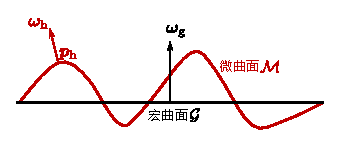
\includegraphics[width=0.6\linewidth]{Pictures/chap08/macrosurfaceMicrosurface.eps}
    \caption{宏曲面(黑色)与微曲面(红色)。}
    \label{fig:08ex01-macrosurfaceMicrosurface}
\end{figure}

我们可以把${\bm\omega}_{\mathrm{m}}$视作从$\mathcal{M}$到整个方向空间$\varOmega$的映射。
注意$\varOmega$包含了球心到完整球面上任意一点的所有可能方向(总立体角为$4\pi$,尽管该映射不一定能覆盖全)。
现在考虑$\mathcal{M}$和$\varOmega$各自的子集$\mathcal{M'}$和$\varOmega'$,
并设它们满足以下条件:点${\bm p}_{\mathrm{m}}$属于$\mathcal{M'}$当且仅当
该点处的微面法线${\bm\omega}_{\mathrm{m}}({\bm p}_{\mathrm{m}})$属于$\varOmega'$,即
\begin{align}
    {\bm p}_{\mathrm{m}}\in\mathcal{M'}\Leftrightarrow{\bm\omega}_{\mathrm{m}}({\bm p}_{\mathrm{m}})\in\varOmega'\, .
\end{align}
由此利用积分换元可得微面分布函数具有计算指定微曲面面积的能力:
\begin{align}
    \label{eq:08ex01-microsurfaceArea}
    \int\limits_{\mathcal{M}'}\mathrm{d}{\bm p}_{\mathrm{m}}=S\int\limits_{\varOmega'}D({\bm\omega}_{\mathrm{m}})\mathrm{d}{\bm\omega}_{\mathrm{m}}\, .
\end{align}
而整个微曲面面积就是
\begin{align}
    \int\limits_{\mathcal{M}}\mathrm{d}{\bm p}_{\mathrm{m}}=S\int\limits_{\varOmega}D({\bm\omega}_{\mathrm{m}})\mathrm{d}{\bm\omega}_{\mathrm{m}}\, .
\end{align}

进一步地,对于任意关于微面法线的函数$f({\bm\omega}_{\mathrm{m}})$,
利用$D({\bm\omega})$可将空间积分与统计积分相互转化:
\begin{align}
    \int\limits_{\mathcal{M}}f({\bm\omega}_{\mathrm{m}}({\bm p}_{\mathrm{m}}))\mathrm{d}{\bm p}_{\mathrm{m}}=S\int\limits_{\varOmega}f({\bm\omega}_{\mathrm{m}})D({\bm\omega}_{\mathrm{m}})\mathrm{d}{\bm\omega}_{\mathrm{m}}\, .
\end{align}

反之,对于任意定义在$\mathcal{M}$上的函数$g({\bm p}_{\mathrm{m}})$,
我们可以定义对应的统计函数$g({\bm\omega}_{\mathrm{m}})$为
\sidenote{这里原论文为了在记号上强调二者的联系,仍然使用了符号$g$,
但读者应明白这是一个新的函数了。后面\refeq{08ex01-StaticMaskFunc}等的情况类似。}:
\begin{align}\label{eq:08ex01-StaticFunc}
    g({\bm\omega})=\frac{\displaystyle\int\limits_{\mathcal{M}}\delta_{\bm\omega}({\bm\omega}_{\mathrm{m}}({\bm p}_{\mathrm{m}}))g({\bm p}_{\mathrm{m}})\mathrm{d}{\bm p}_{\mathrm{m}}}{\displaystyle\int\limits_{\mathcal{M}}\delta_{\bm\omega}({\bm\omega}_{\mathrm{m}}({\bm p}_{\mathrm{m}}))\mathrm{d}{\bm p}_{\mathrm{m}}}\, .
\end{align}
该函数也可以实现空间积分与统计积分的相互转化:
\begin{align}\label{eq:08ex01-TransferSpaceStatic}
    \int\limits_{\mathcal{M}}g({\bm p}_{\mathrm{m}})\mathrm{d}{\bm p}_{\mathrm{m}}=S\int\limits_{\varOmega}g({\bm\omega}_{\mathrm{m}})D({\bm\omega}_{\mathrm{m}})\mathrm{d}{\bm\omega}_{\mathrm{m}}\, .
\end{align}

如\reffig{08ex01-ProjectionsMicrofacetArea},理解以上推导后,我们可以计算以下面积。
\begin{figure}[htbp]
    \centering
    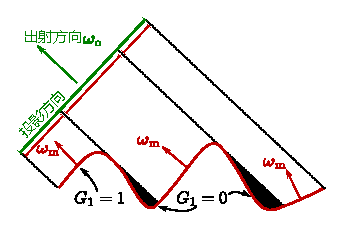
\includegraphics[width=0.5\linewidth]{Pictures/chap08/ProjectionsMicrofacet.eps}
    \caption{微面可见部分在${\bm\omega}_{\mathrm{o}}$上的投影面积。}
    \label{fig:08ex01-ProjectionsMicrofacetArea}
\end{figure}

首先,微曲面在宏曲面法线方向${\bm\omega}_{\mathrm{g}}$上的
投影面积(不论是否遮挡,且背向时记负值)为
\begin{align}
    \int\limits_{\mathcal{M}}({\bm\omega}_{\mathrm{m}}({\bm p}_{\mathrm{m}})\cdot{\bm\omega}_{\mathrm{g}})\mathrm{d}{\bm p}_{\mathrm{m}}=S\int\limits_{\varOmega}({\bm\omega}_{\mathrm{m}}\cdot{\bm\omega}_{\mathrm{g}})D({\bm\omega}_{\mathrm{m}})\mathrm{d}{\bm\omega}_{\mathrm{m}}=\int\limits_{\mathcal{G}}\mathrm{d}{\bm p}_{\mathrm{g}}=S\, .
\end{align}

接着我们从出射方向${\bm\omega}_{\mathrm{o}}$来观察曲面。此时宏曲面在${\bm\omega}_{\mathrm{o}}$上的投影面积为
\begin{align}
    \label{eq:08ex01-AreaMacrosurface}
    ({\bm\omega}_{\mathrm{o}}\cdot{\bm\omega}_{\mathrm{g}})S=S\cos\theta_{\mathrm{o}}\, ,
\end{align}
其中$\theta_{\mathrm{o}}$为${\bm\omega}_{\mathrm{o}}$与${\bm\omega}_{\mathrm{g}}$的夹角。

最后我们算得微面可见部分在${\bm\omega}_{\mathrm{o}}$上的投影面积为
\begin{align}\label{eq:08ex01-AreaProjectionsMicrofacetVisible}
    \int\limits_{\mathcal{M}}G_1({\bm\omega}_{\mathrm{o}},{\bm p}_{\mathrm{m}})\max({\bm\omega}_{\mathrm{o}}\cdot{\bm\omega}_{\mathrm{m}}({\bm p}_{\mathrm{m}}),0)\mathrm{d}{\bm p}_{\mathrm{m}}\, ,
\end{align}
其中空间掩膜函数$G_1({\bm\omega}_{\mathrm{o}},{\bm p}_{\mathrm{m}})$在${\bm p}_{\mathrm{m}}$被
遮挡时取0,否则取1. 而$\max$项则过滤了背向不可见的微面。
其对应的统计掩膜函数$G_1({\bm\omega}_{\mathrm{o}},{\bm\omega}_{\mathrm{m}})$的值域为$[0,1]$,
它给出了从方向${\bm\omega}_{\mathrm{o}}$观察时,法线为${\bm\omega}_{\mathrm{m}}$的微面中可见的比例:
\begin{align}\label{eq:08ex01-StaticMaskFunc}
    G_1({\bm\omega}_{\mathrm{o}},{\bm\omega})=\frac{\displaystyle\int\limits_{\mathcal{M}}\delta_{\bm\omega}({\bm\omega}_{\mathrm{m}}({\bm p}_{\mathrm{m}}))G_1({\bm\omega}_{\mathrm{o}},{\bm p}_{\mathrm{m}})\mathrm{d}{\bm p}_{\mathrm{m}}}{\displaystyle\int\limits_{\mathcal{M}}\delta_{\bm\omega}({\bm\omega}_{\mathrm{m}}({\bm p}_{\mathrm{m}}))\mathrm{d}{\bm p}_{\mathrm{m}}}\, .
\end{align}
由此得到投影面积的另一计算方式:
\begin{align}
    \label{eq:08ex01-AreaMicrosurface}
    S\int\limits_{\varOmega}G_1({\bm\omega}_{\mathrm{o}},{\bm\omega}_{\mathrm{m}})\max({\bm\omega}_{\mathrm{o}}\cdot{\bm\omega}_{\mathrm{m}},0)D({\bm\omega}_{\mathrm{m}})\mathrm{d}{\bm\omega}_{\mathrm{m}}\, .
\end{align}

由于可见微面投影面积等于宏曲面投影面积,所以
结合\refeq{08ex01-AreaMacrosurface}和\refeq{08ex01-AreaMicrosurface}可得
基于物理的掩膜函数$G_1$总是满足如下约束:
\begin{align}
    \cos\theta_{\mathrm{o}}=\int\limits_{\varOmega}G_1({\bm\omega}_{\mathrm{o}},{\bm\omega}_{\mathrm{m}})\max({\bm\omega}_{\mathrm{o}}\cdot{\bm\omega}_{\mathrm{m}},0)D({\bm\omega}_{\mathrm{m}})\mathrm{d}{\bm\omega}_{\mathrm{m}}\, .
\end{align}
注意这并不意味着该约束唯一确定了$G_1$,它常常有无数个解。
还需引入其他约束或假设才能限定为唯一解。

此外,译者再补充两个\refeq{08ex01-StaticMaskFunc}可能让人感到困惑的地方:

第一个是记号的问题。$G_1({\bm\omega}_{\mathrm{o}},{\bm\omega}_{\mathrm{m}})$中
第二个自变量是${\bm\omega}_{\mathrm{m}}$,该变量应出现在其定义式中狄拉克$\delta$分布的下标,
但狄拉克$\delta$分布后面的括号内还有一个记号相同的函数${\bm\omega}_{\mathrm{m}}({\bm p}_{\mathrm{m}})$,
所以为了区分它们,\refeq{08ex01-StaticMaskFunc}中临时把第二个自变量改写为${\bm\omega}$.
笔者保留了原论文的这个做法,请读者注意区分。
\refeq{08ex01-StaticFunc}和\refeq{08ex01-AnotherStaticFunc}也用了类似的临时记号。

第二个是定义的问题。细心的读者可能注意到,
比对\refeq{08ex01-AreaProjectionsMicrofacetVisible}和\refeq{08ex01-TransferSpaceStatic},
我们本该设
\begin{align}\label{eq:08ex01-AnotherSpaceFunc}
    g({\bm p}_{\mathrm{m}})=G_1({\bm\omega}_{\mathrm{o}},{\bm p}_{\mathrm{m}})\max({\bm\omega}_{\mathrm{o}}\cdot{\bm\omega}_{\mathrm{m}}({\bm p}_{\mathrm{m}}),0)\, ,
\end{align}
此时使得\refeq{08ex01-TransferSpaceStatic}成立的$g({\bm\omega}_{\mathrm{m}})$应该是
把\refeq{08ex01-AnotherSpaceFunc}带入\refeq{08ex01-StaticFunc}得到的
\begin{align}\label{eq:08ex01-AnotherStaticFunc}
    g({\bm\omega})=\frac{\displaystyle\int\limits_{\mathcal{M}}\delta_{\bm\omega}({\bm\omega}_{\mathrm{m}}({\bm p}_{\mathrm{m}}))G_1({\bm\omega}_{\mathrm{o}},{\bm p}_{\mathrm{m}})\max({\bm\omega}_{\mathrm{o}}\cdot{\bm\omega}_{\mathrm{m}}({\bm p}_{\mathrm{m}}),0)\mathrm{d}{\bm p}_{\mathrm{m}}}{\displaystyle\int\limits_{\mathcal{M}}\delta_{\bm\omega}({\bm\omega}_{\mathrm{m}}({\bm p}_{\mathrm{m}}))\mathrm{d}{\bm p}_{\mathrm{m}}}\, .
\end{align}
将上式回代\refeq{08ex01-TransferSpaceStatic}的右边后,
读者会发现它和\refeq{08ex01-AreaMicrosurface}并不是完全一样的——
后者相当于把前者内层积分中的项$\max({\bm\omega}_{\mathrm{o}}\cdot{\bm\omega}_{\mathrm{m}}({\bm p}_{\mathrm{m}}),0)$
(里面的${\bm\omega}_{\mathrm{m}}$是函数)提到外层积分中
变成了$\max({\bm\omega}_{\mathrm{o}}\cdot{\bm\omega}_{\mathrm{m}},0)$
(里面的${\bm\omega}_{\mathrm{m}}$是变量)。
一般来说积分变量并不能随便外提,但因为这里内层积分中含有狄拉克$\delta$分布,
它使得此处外提$\max$项的做法恰好没有改变整个式子的值。
所以原论文中作出简化处理,相当于令$g({\bm p}_{\mathrm{m}})=G_1({\bm\omega}_{\mathrm{o}},{\bm p}_{\mathrm{m}})$,
此时对应的$g({\bm\omega}_{\mathrm{m}})$即为\refeq{08ex01-StaticMaskFunc}中
的$G_1({\bm\omega}_{\mathrm{o}},{\bm\omega}_{\mathrm{m}})$.
不过原作者并未交代这样的细节。

\subsection{典型微面分布函数的规范性证明}\label{sub:典型微面分布函数的规范性证明}
本节补充了\refeq{8.10}和\refeq{8.11}所给的
微面分布函数$D({\bm\omega}_{\mathrm{h}})$满足规范性要求的证明,即证明
\begin{align}\label{eq:8.ex-01}
    \int\limits_{H^2({\bm n})}D({\bm\omega}_{\mathrm{h}})\cos\theta_{\mathrm{h}}\mathrm{d}{\bm\omega}_{\mathrm{h}}=1\, .
\end{align}

为了简化证明过程,我们先证明以下积分式(其中$\alpha_x,\alpha_y>0$):
\begin{align}\label{eq:8.ex-02}
    \int_{\varphi_{\mathrm{h}}=0}^{2\pi}\frac{1}{2\pi\alpha_x\alpha_y\left(\frac{\cos^2\varphi_{\mathrm{h}}}{\alpha_x^2}+\frac{\sin^2\varphi_{\mathrm{h}}}{\alpha_y^2}\right)}\mathrm{d}\varphi_{\mathrm{h}}=1\, .
\end{align}
\begin{prove}
    \begin{align}
                                                         & \int_{\varphi_{\mathrm{h}}=0}^{2\pi}\frac{1}{2\pi\alpha_x\alpha_y\left(\frac{\cos^2\varphi_{\mathrm{h}}}{\alpha_x^2}+\frac{\sin^2\varphi_{\mathrm{h}}}{\alpha_y^2}\right)}\mathrm{d}\varphi_{\mathrm{h}}\nonumber \\
        =                                                & \int_{\varphi_{\mathrm{h}}=0}^{2\pi}\frac{\alpha_x\alpha_y}{2\pi(\alpha_x^2\sin^2\varphi_{\mathrm{h}}+\alpha_y^2\cos^2\varphi_{\mathrm{h}})}\mathrm{d}\varphi_{\mathrm{h}}\nonumber                               \\
        =                                                & \frac{\alpha_x\alpha_y}{2\pi}\int_{\varphi_{\mathrm{h}}=0}^{2\pi}\frac{1}{(\alpha_x^2\tan^2\varphi_{\mathrm{h}}+\alpha_y^2)\cos^2\varphi_{\mathrm{h}}}\mathrm{d}\varphi_{\mathrm{h}}\nonumber                     \\
        =                                                & \frac{\alpha_x\alpha_y}{\pi}\int_{\varphi_{\mathrm{h}}=0}^{\pi}\frac{1}{\alpha_x^2\tan^2\varphi_{\mathrm{h}}+\alpha_y^2}\mathrm{d}\tan\varphi_{\mathrm{h}}\nonumber                                               \\
        =                                                & \frac{\alpha_x\alpha_y}{\pi}\int_{\varphi_{\mathrm{h}}=-\frac{\pi}{2}}^{\frac{\pi}{2}}\frac{1}{\alpha_x^2\tan^2\varphi_{\mathrm{h}}+\alpha_y^2}\mathrm{d}\tan\varphi_{\mathrm{h}}\nonumber                        \\
        \xlongequal{\text{令}t=\tan\varphi_{\mathrm{h}}} & \frac{\alpha_x\alpha_y}{\pi}\int_{t=-\infty}^{+\infty}\frac{1}{\alpha_x^2t^2+\alpha_y^2}\mathrm{d}t\nonumber                                                                                                      \\
        =                                                & \frac{1}{\pi}\int_{t=-\infty}^{+\infty}\frac{1}{\left(\frac{\alpha_xt}{\alpha_y}\right)^2+1}\mathrm{d}\frac{\alpha_xt}{\alpha_y}\nonumber                                                                         \\
        =                                                & \frac{1}{\pi}\arctan\frac{\alpha_xt}{\alpha_y}\bigg|_{t=-\infty}^{+\infty}\nonumber                                                                                                                               \\
        =                                                & 1\, .
    \end{align}
\end{prove}

接下来证明各向异性的Beckmann-Spizzichino模型即\refeq{8.10}满足规范性。
\begin{prove}
    设
    \begin{align}\label{eq:8.ex-03}
        \beta=\frac{\cos^2\varphi_{\mathrm{h}}}{\alpha_x^2}+\frac{\sin^2\varphi_{\mathrm{h}}}{\alpha_y^2}>0\quad(\alpha_x,\alpha_y>0)\, .
    \end{align}
    利用上述变量简化积分并结合\refeq{8.ex-02},可得
    \begin{align}
          & \int\limits_{H^2({\bm n})}D({\bm\omega}_{\mathrm{h}})\cos\theta_{\mathrm{h}}\mathrm{d}{\bm\omega}_{\mathrm{h}}\nonumber                                                                                                                                                                                                                                                         \\
        = & \int\limits_{H^2({\bm n})}\frac{\mathrm{e}^{-\left(\frac{\cos^2\varphi_{\mathrm{h}}}{\alpha_x^2}+\frac{\sin^2\varphi_{\mathrm{h}}}{\alpha_y^2}\right)\tan^2\theta_{\mathrm{h}}}}{\pi\alpha_x\alpha_y\cos^4\theta_{\mathrm{h}}}\cos\theta_{\mathrm{h}}\mathrm{d}{\bm\omega}_{\mathrm{h}}\nonumber                                                                                \\
        = & \int_{\varphi_{\mathrm{h}}=0}^{2\pi}\int_{\theta_{\mathrm{h}}=0}^{\frac{\pi}{2}}\frac{\mathrm{e}^{-\left(\frac{\cos^2\varphi_{\mathrm{h}}}{\alpha_x^2}+\frac{\sin^2\varphi_{\mathrm{h}}}{\alpha_y^2}\right)\tan^2\theta_{\mathrm{h}}}}{\pi\alpha_x\alpha_y\cos^3\theta_{\mathrm{h}}}\sin\theta_{\mathrm{h}}\mathrm{d}\theta_{\mathrm{h}}\mathrm{d}\varphi_{\mathrm{h}}\nonumber \\
        = & \int_{\varphi_{\mathrm{h}}=0}^{2\pi}\int_{\theta_{\mathrm{h}}=0}^{\frac{\pi}{2}}\frac{\tan\theta_{\mathrm{h}}}{\pi\alpha_x\alpha_y\cos^2\theta_{\mathrm{h}}}\mathrm{e}^{-\beta \tan^2\theta_{\mathrm{h}}}\mathrm{d}\theta_{\mathrm{h}}\mathrm{d}\varphi_{\mathrm{h}}\nonumber                                                                                                   \\
        = & \int_{\varphi_{\mathrm{h}}=0}^{2\pi}\int_{\theta_{\mathrm{h}}=0}^{\frac{\pi}{2}}\frac{-1}{2\pi\alpha_x\alpha_y\beta}\mathrm{d}\mathrm{e}^{-\beta \tan^2\theta_{\mathrm{h}}}\mathrm{d}\varphi_{\mathrm{h}}\nonumber                                                                                                                                                              \\
        = & \int_{\varphi_{\mathrm{h}}=0}^{2\pi}\frac{-1}{2\pi\alpha_x\alpha_y\beta}\left(\mathrm{e}^{-\beta \tan^2\theta_{\mathrm{h}}}\bigg|_{\theta_{\mathrm{h}}=0}^{\frac{\pi}{2}}\right)\mathrm{d}\varphi_{\mathrm{h}}\nonumber                                                                                                                                                         \\
        = & \int_{\varphi_{\mathrm{h}}=0}^{2\pi}\frac{1}{2\pi\alpha_x\alpha_y\beta}\mathrm{d}\varphi_{\mathrm{h}}\nonumber                                                                                                                                                                                                                                                                  \\
        = & 1\, .
    \end{align}
\end{prove}

Trowbridge-Reitz模型即\refeq{8.11}的证明是类似的。
\begin{prove}
    同样按\refeq{8.ex-03}设好$\beta$,结合\refeq{8.ex-02},可得
    \begin{align}
                                                                 & \int\limits_{H^2({\bm n})}D({\bm\omega}_{\mathrm{h}})\cos\theta_{\mathrm{h}}\mathrm{d}{\bm\omega}_{\mathrm{h}}\nonumber                                                                                                                                                                                                                                                            \\
        =                                                        & \int\limits_{H^2({\bm n})}\frac{1}{\pi\alpha_x\alpha_y\left(1+\left(\frac{\cos^2\varphi_{\mathrm{h}}}{\alpha_x^2}+\frac{\sin^2\varphi_{\mathrm{h}}}{\alpha_y^2}\right)\tan^2\theta_{\mathrm{h}}\right)^2\cos^4\theta_{\mathrm{h}}}\cos\theta_{\mathrm{h}}\mathrm{d}{\bm\omega}_{\mathrm{h}}\nonumber                                                                               \\
        =                                                        & \int_{\varphi_{\mathrm{h}}=0}^{2\pi}\int_{\theta_{\mathrm{h}}=0}^{\frac{\pi}{2}}\frac{\sin\theta_{\mathrm{h}}}{\pi\alpha_x\alpha_y\left(1+\left(\frac{\cos^2\varphi_{\mathrm{h}}}{\alpha_x^2}+\frac{\sin^2\varphi_{\mathrm{h}}}{\alpha_y^2}\right)\tan^2\theta_{\mathrm{h}}\right)^2\cos^3\theta_{\mathrm{h}}}\mathrm{d}\theta_{\mathrm{h}}\mathrm{d}\varphi_{\mathrm{h}}\nonumber \\
        =                                                        & \int_{\varphi_{\mathrm{h}}=0}^{2\pi}\int_{\theta_{\mathrm{h}}=0}^{\frac{\pi}{2}}\frac{\tan\theta_{\mathrm{h}}}{\pi\alpha_x\alpha_y(1+\beta\tan^2\theta_{\mathrm{h}})^2\cos^2\theta_{\mathrm{h}}}\mathrm{d}\theta_{\mathrm{h}}\mathrm{d}\varphi_{\mathrm{h}}\nonumber                                                                                                               \\
        =                                                        & \int_{\varphi_{\mathrm{h}}=0}^{2\pi}\int_{\theta_{\mathrm{h}}=0}^{\frac{\pi}{2}}\frac{1}{2\pi\alpha_x\alpha_y\beta(1+\beta\tan^2\theta_{\mathrm{h}})^2}\mathrm{d}(\beta\tan^2\theta_{\mathrm{h}})\mathrm{d}\varphi_{\mathrm{h}}\nonumber                                                                                                                                           \\
        \xlongequal{\text{令}u=1+\beta\tan^2\theta_{\mathrm{h}}} & \int_{\varphi_{\mathrm{h}}=0}^{2\pi}\int_{u=1}^{+\infty}\frac{1}{2\pi\alpha_x\alpha_y\beta u^2}\mathrm{d}u\mathrm{d}\varphi_{\mathrm{h}}\nonumber                                                                                                                                                                                                                                  \\
        =                                                        & \int_{\varphi_{\mathrm{h}}=0}^{2\pi}\int_{u=1}^{+\infty}\frac{-1}{2\pi\alpha_x\alpha_y\beta}\mathrm{d}u^{-1}\mathrm{d}\varphi_{\mathrm{h}}\nonumber                                                                                                                                                                                                                                \\
        =                                                        & \int_{\varphi_{\mathrm{h}}=0}^{2\pi}\frac{-1}{2\pi\alpha_x\alpha_y\beta}\left(\frac{1}{u}\bigg|_{u=1}^{+\infty}\right)\mathrm{d}\varphi_{\mathrm{h}}\nonumber                                                                                                                                                                                                                      \\
        =                                                        & \int_{\varphi_{\mathrm{h}}=0}^{2\pi}\frac{1}{2\pi\alpha_x\alpha_y\beta}\mathrm{d}\varphi_{\mathrm{h}}\nonumber                                                                                                                                                                                                                                                                     \\
        =                                                        & 1\, .
    \end{align}
\end{prove}